\documentclass[12pt]{article}

\title{Symbolic Logic HW 6}
\author{Tyler Tracy}

\usepackage{amsmath}
\usepackage{amssymb}
\usepackage{graphicx}
\graphicspath{ {./imgs/} }

\begin{document}

\maketitle

\section*{Problem 1}

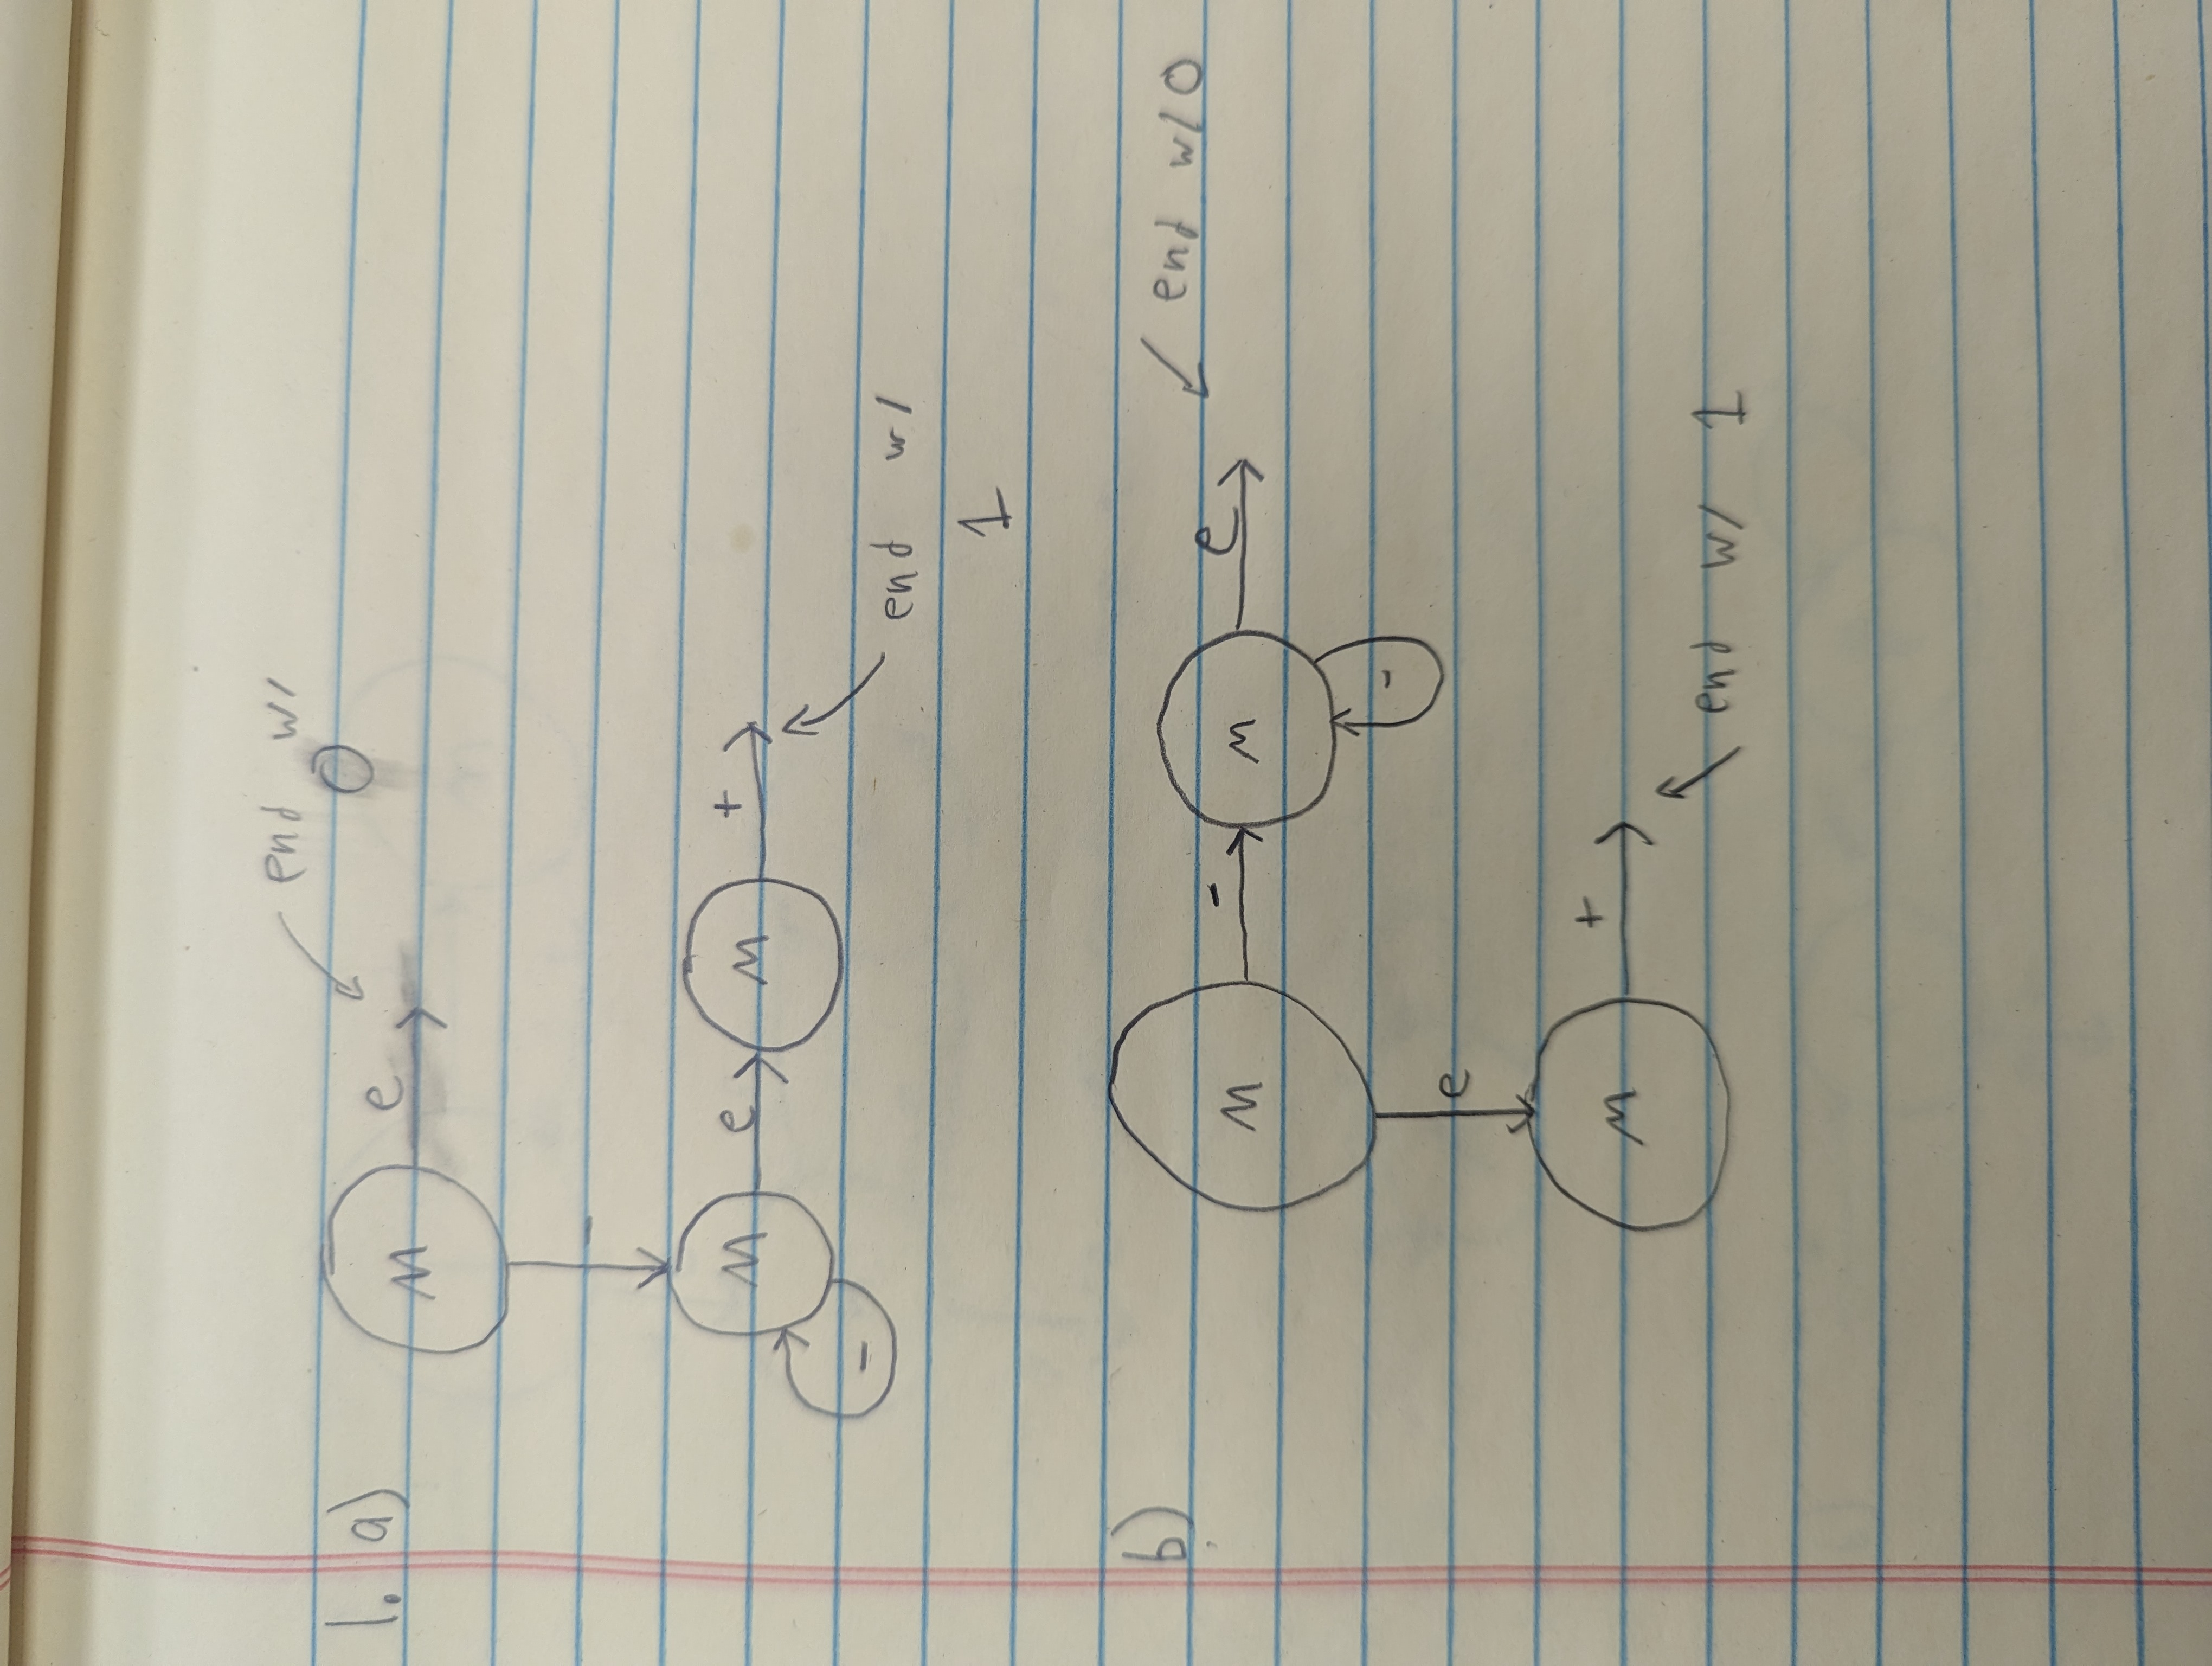
\includegraphics[angle=270,width=\textwidth]{1}

\section*{Problem 2}

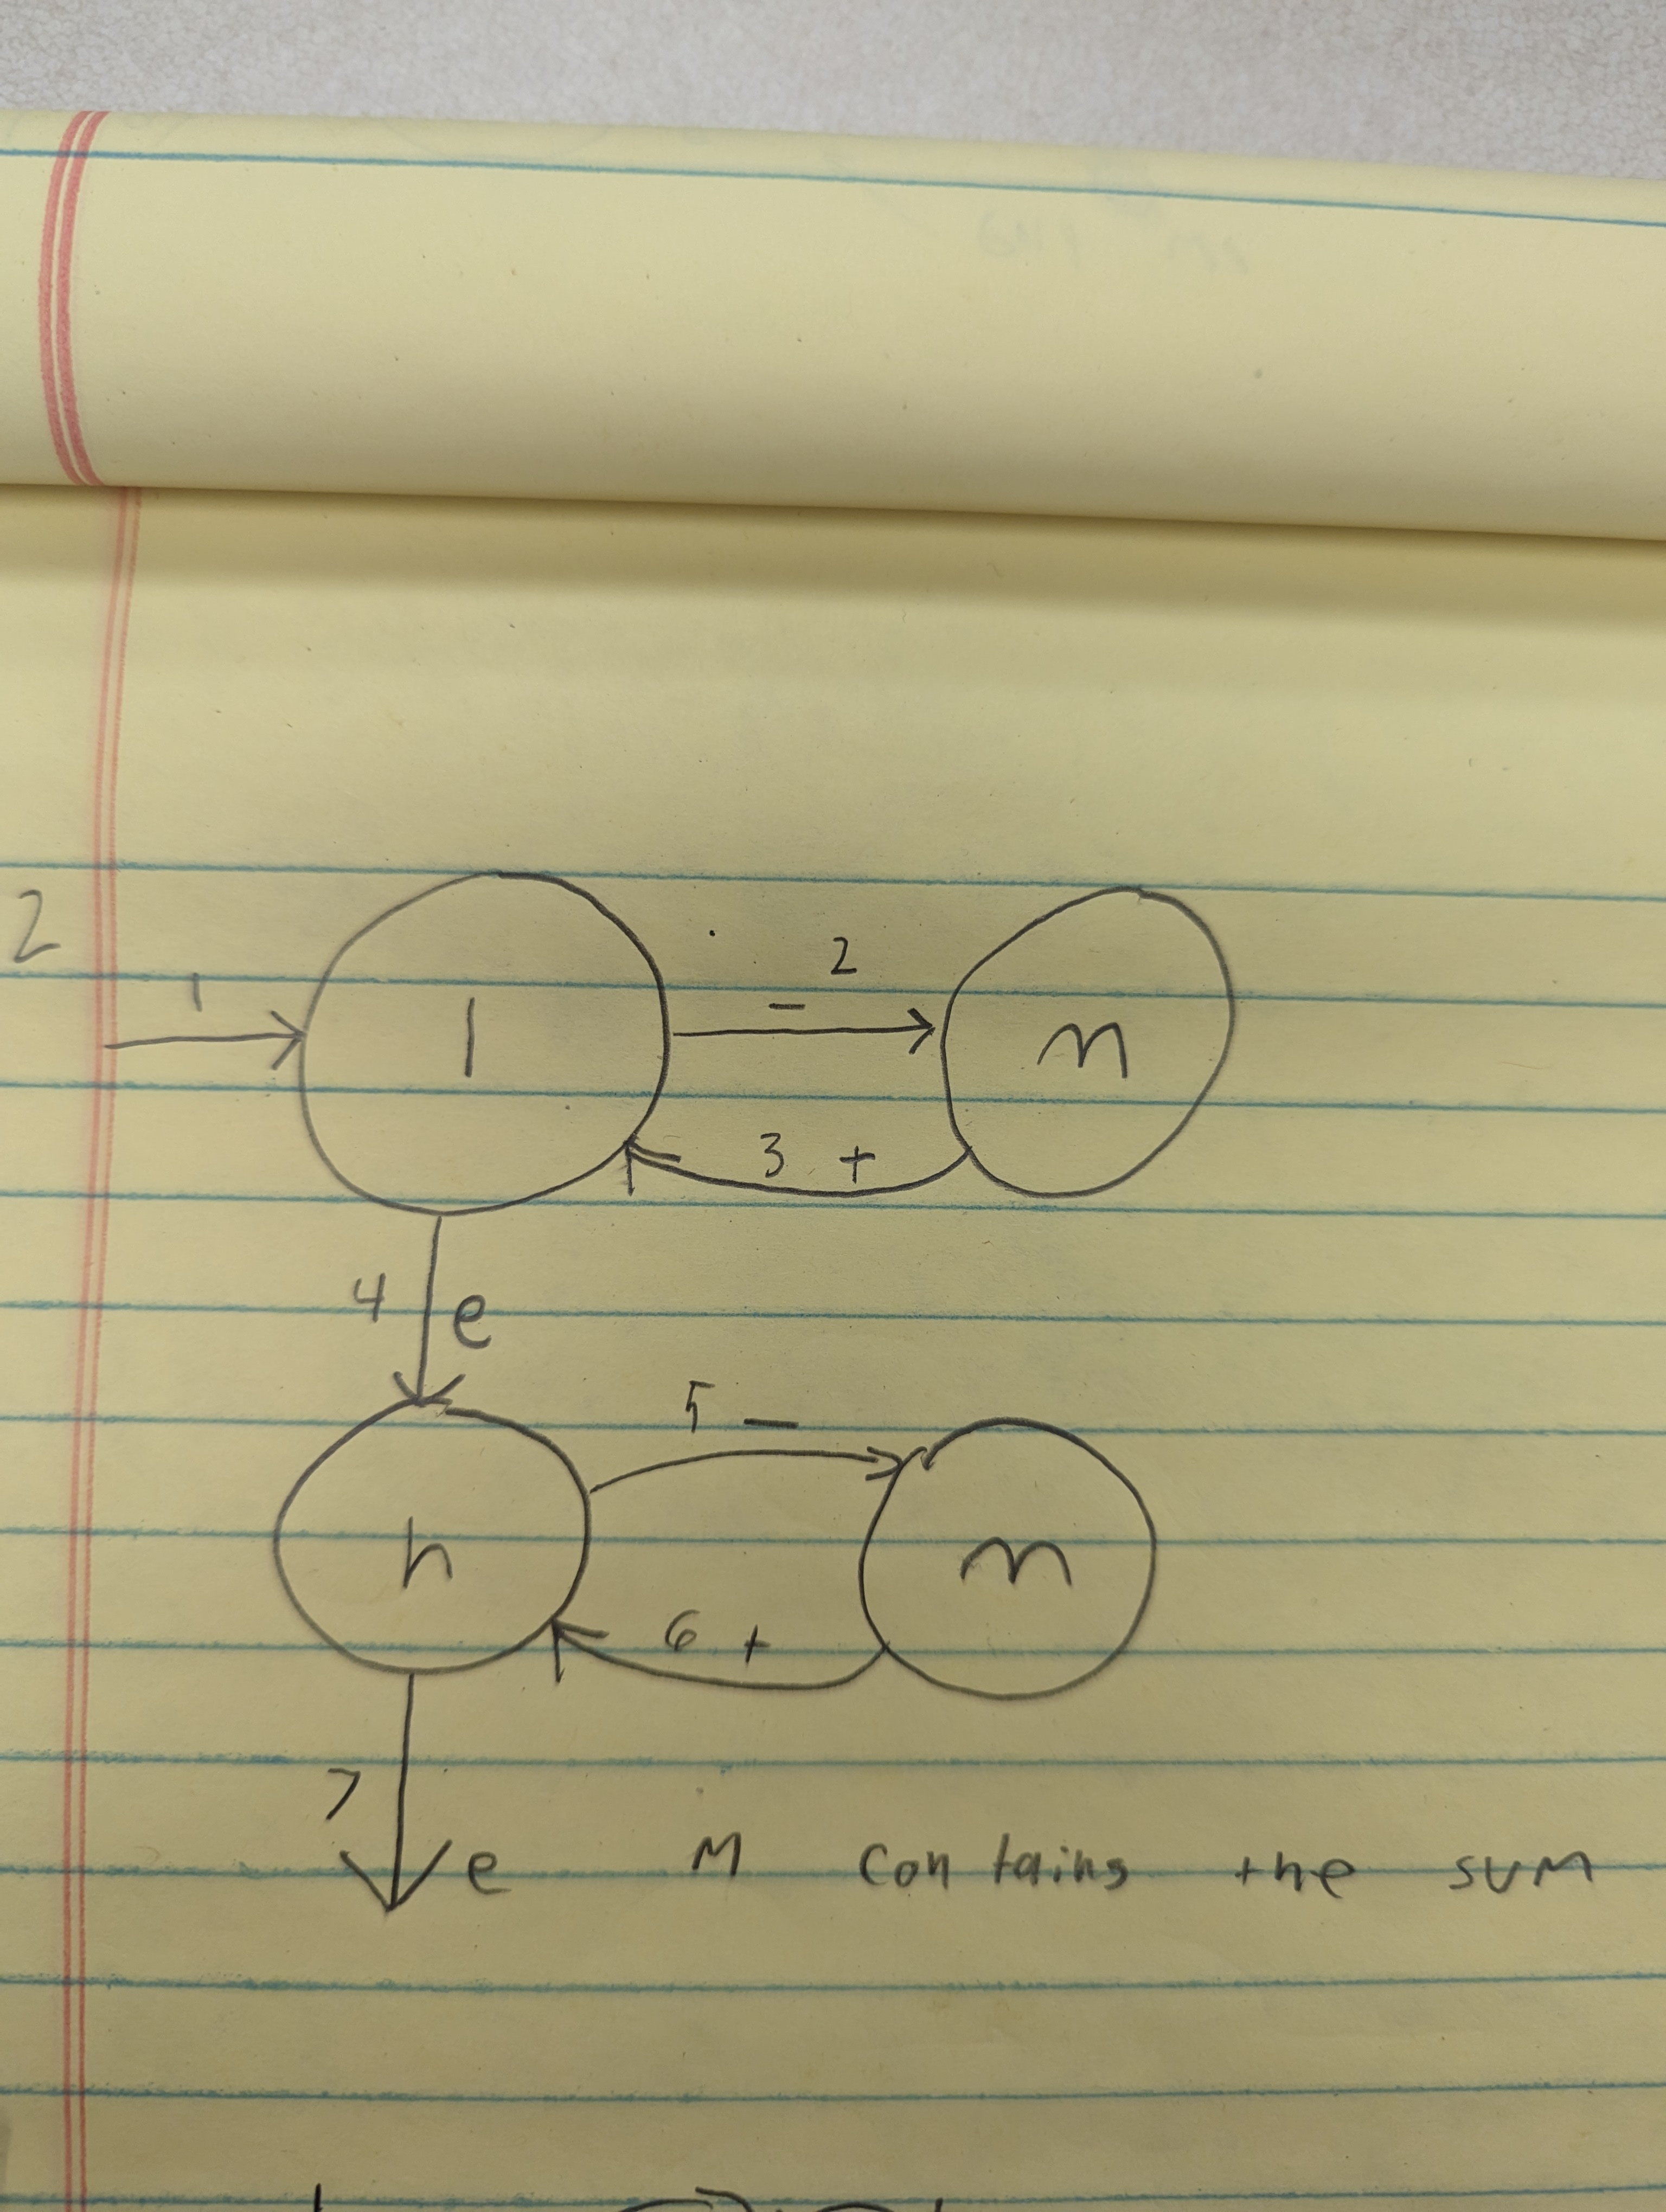
\includegraphics[width=\textwidth]{2}


\section*{Problem 3}

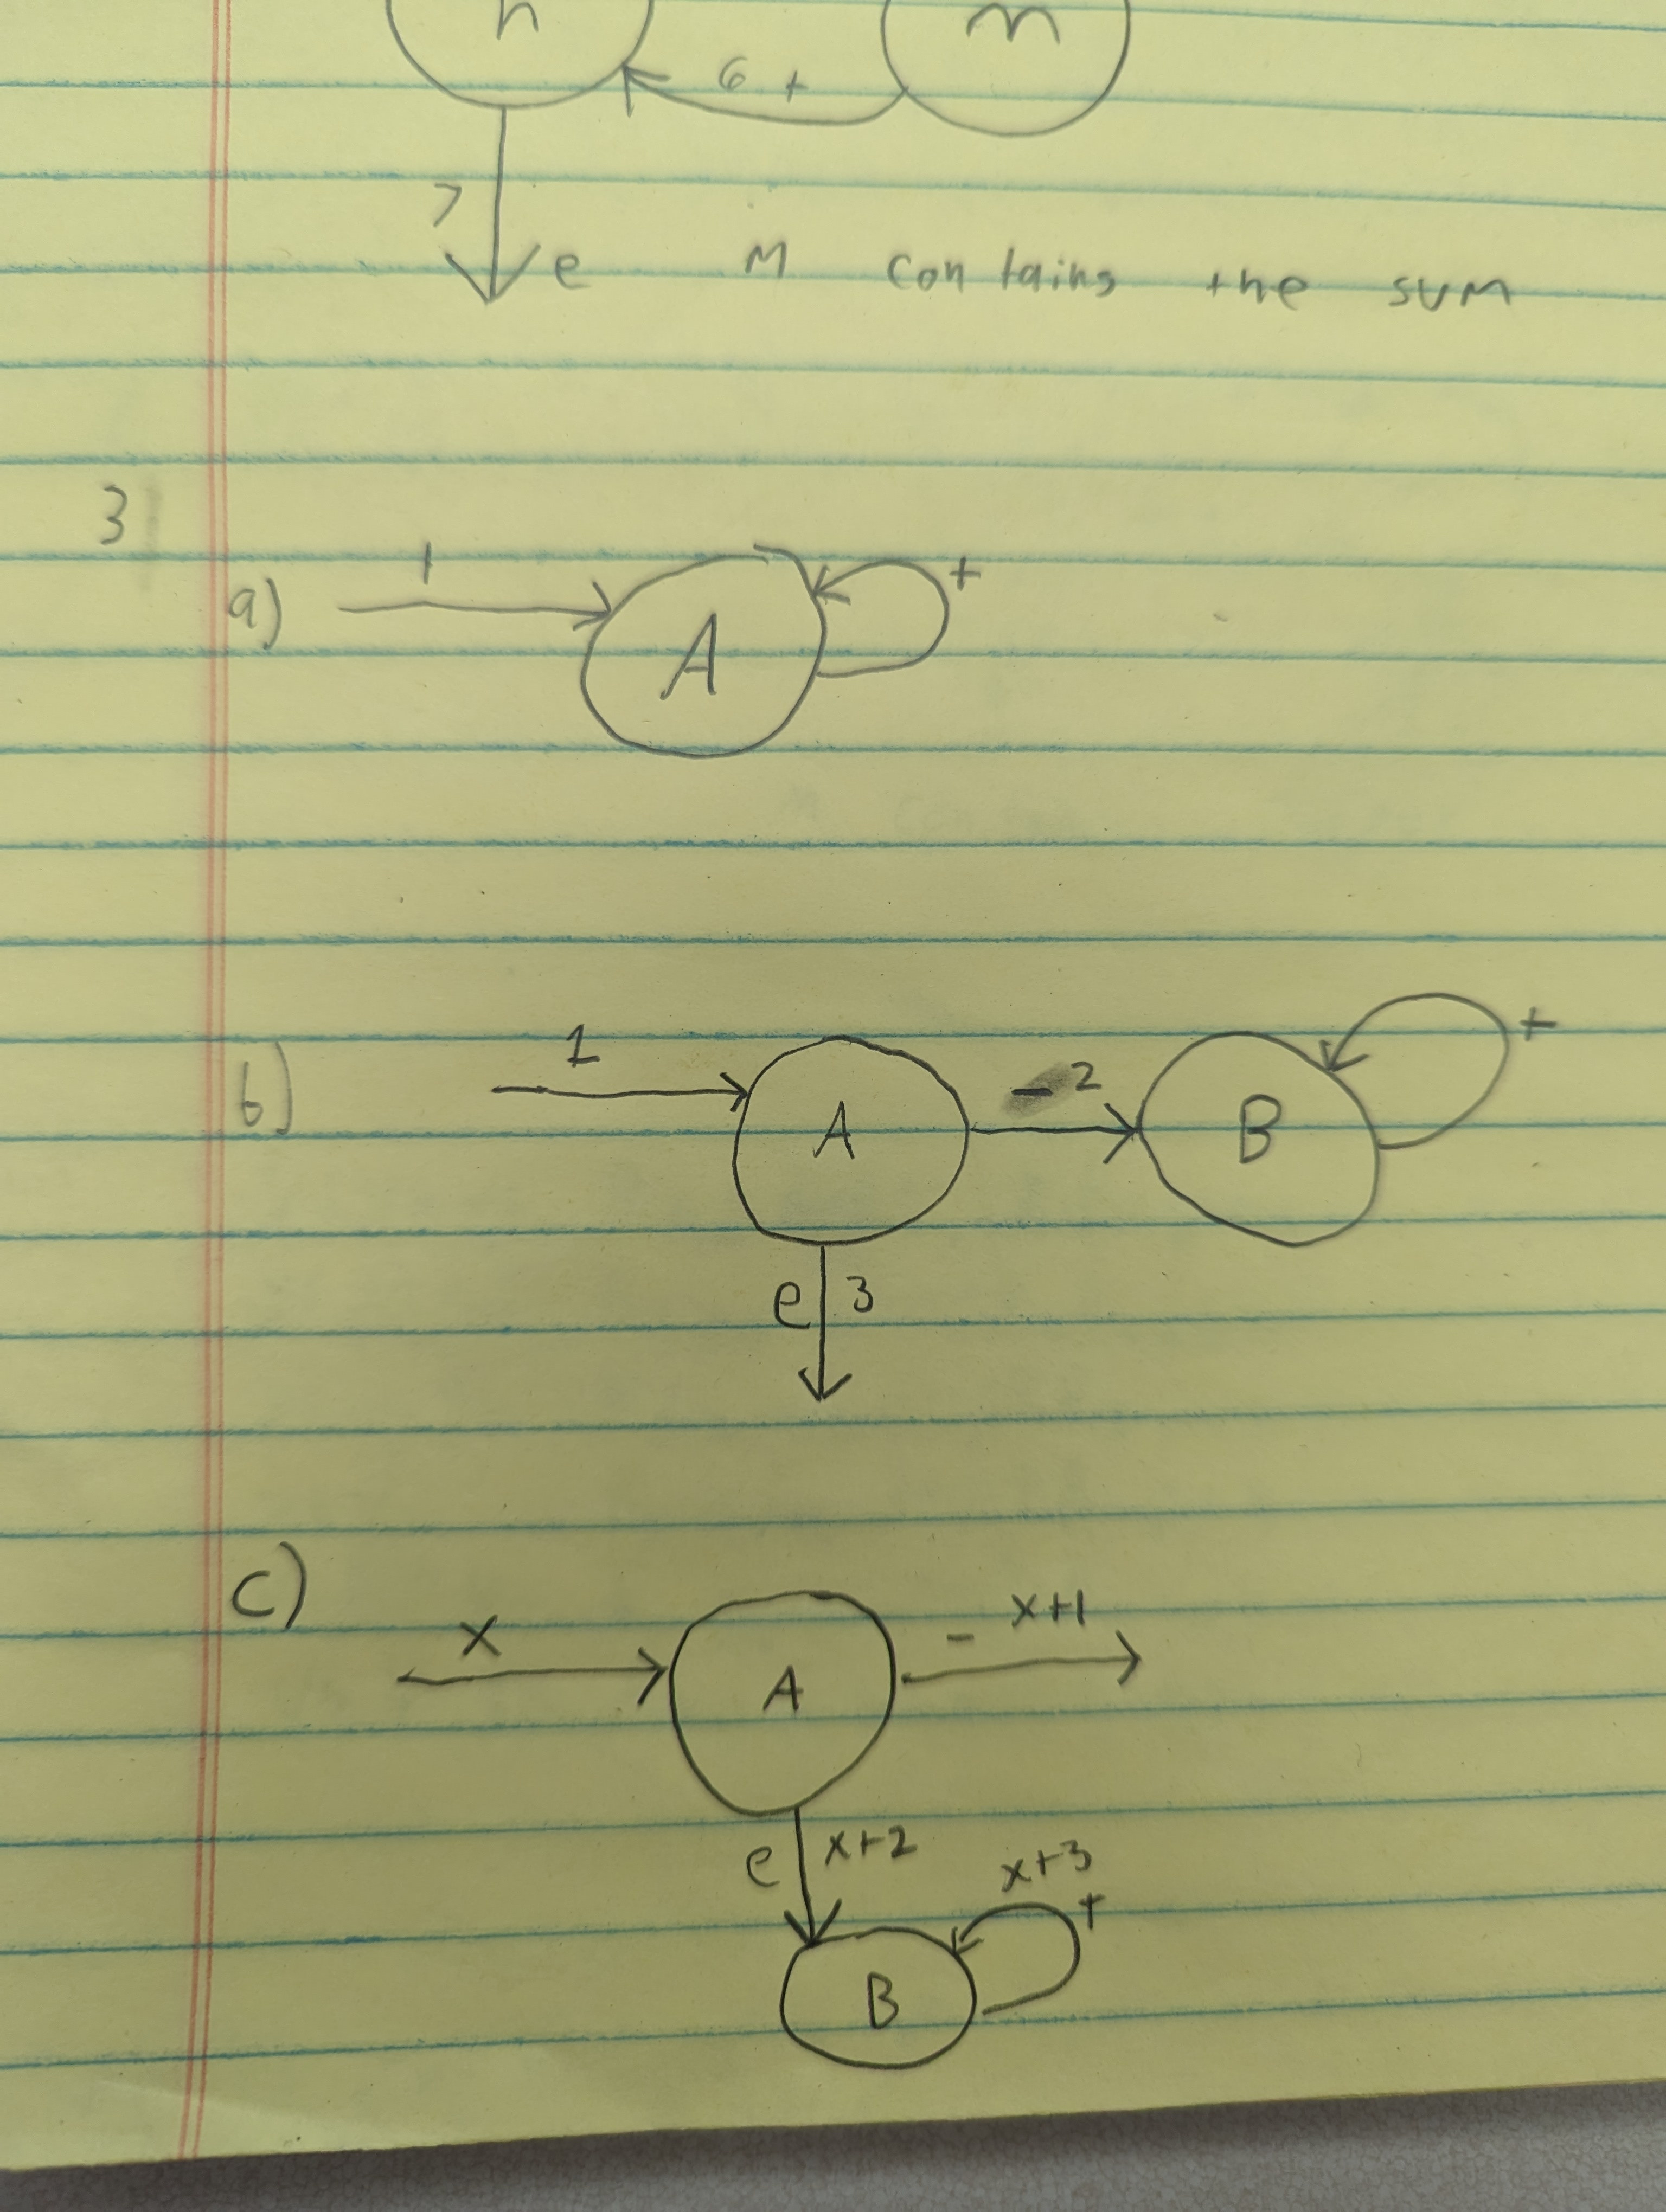
\includegraphics[width=\textwidth]{3}


\section*{Problem 4}


\subsection*{Part A}

Yes, adding the set $\{0, -1, -2, -3, -4, -5\}$ to the counting numbers is enumerably infinite. We can create a mapping from this set to the counting numbers. Each element in this set will be mapped by adding 6 to itself, this will yeild a counting number for every simple element of the set. 


\subsection*{Part B}

There are many more decimal numbers (real numbers) between 0 and 1 than there are counting numbers. We can use a diagonalization argument to show this. Suppose that you give me any enumerable set of real numbers between 0 and 1, I can enumerate all the numbers and create a new number that isn't in the original set. I can do this by ensuring that the new number is different from all the other numbers in at least one location. Starting with the first number, if it begins with a 1, then my number will begin with a 0, if it begins with anything else, then my new number will begin with a 1. This process will be repeated for every single number in the provided set, shifting the index that is examined by 1 for each number. This will ensure that this new number is different from all other numbers. This means that there can not exist an enumerable set of real numbers. 

\subsection*{Part C}

There are many less rational numbers in between 0 and 1 than there are real numbers. Rational numbers can express irrational numbers like the square root of two. Thus, a diagonalization argument can't apply because I can't create a new rational number by flipping the digits of other rational numbers. 


\section*{Problem 5}

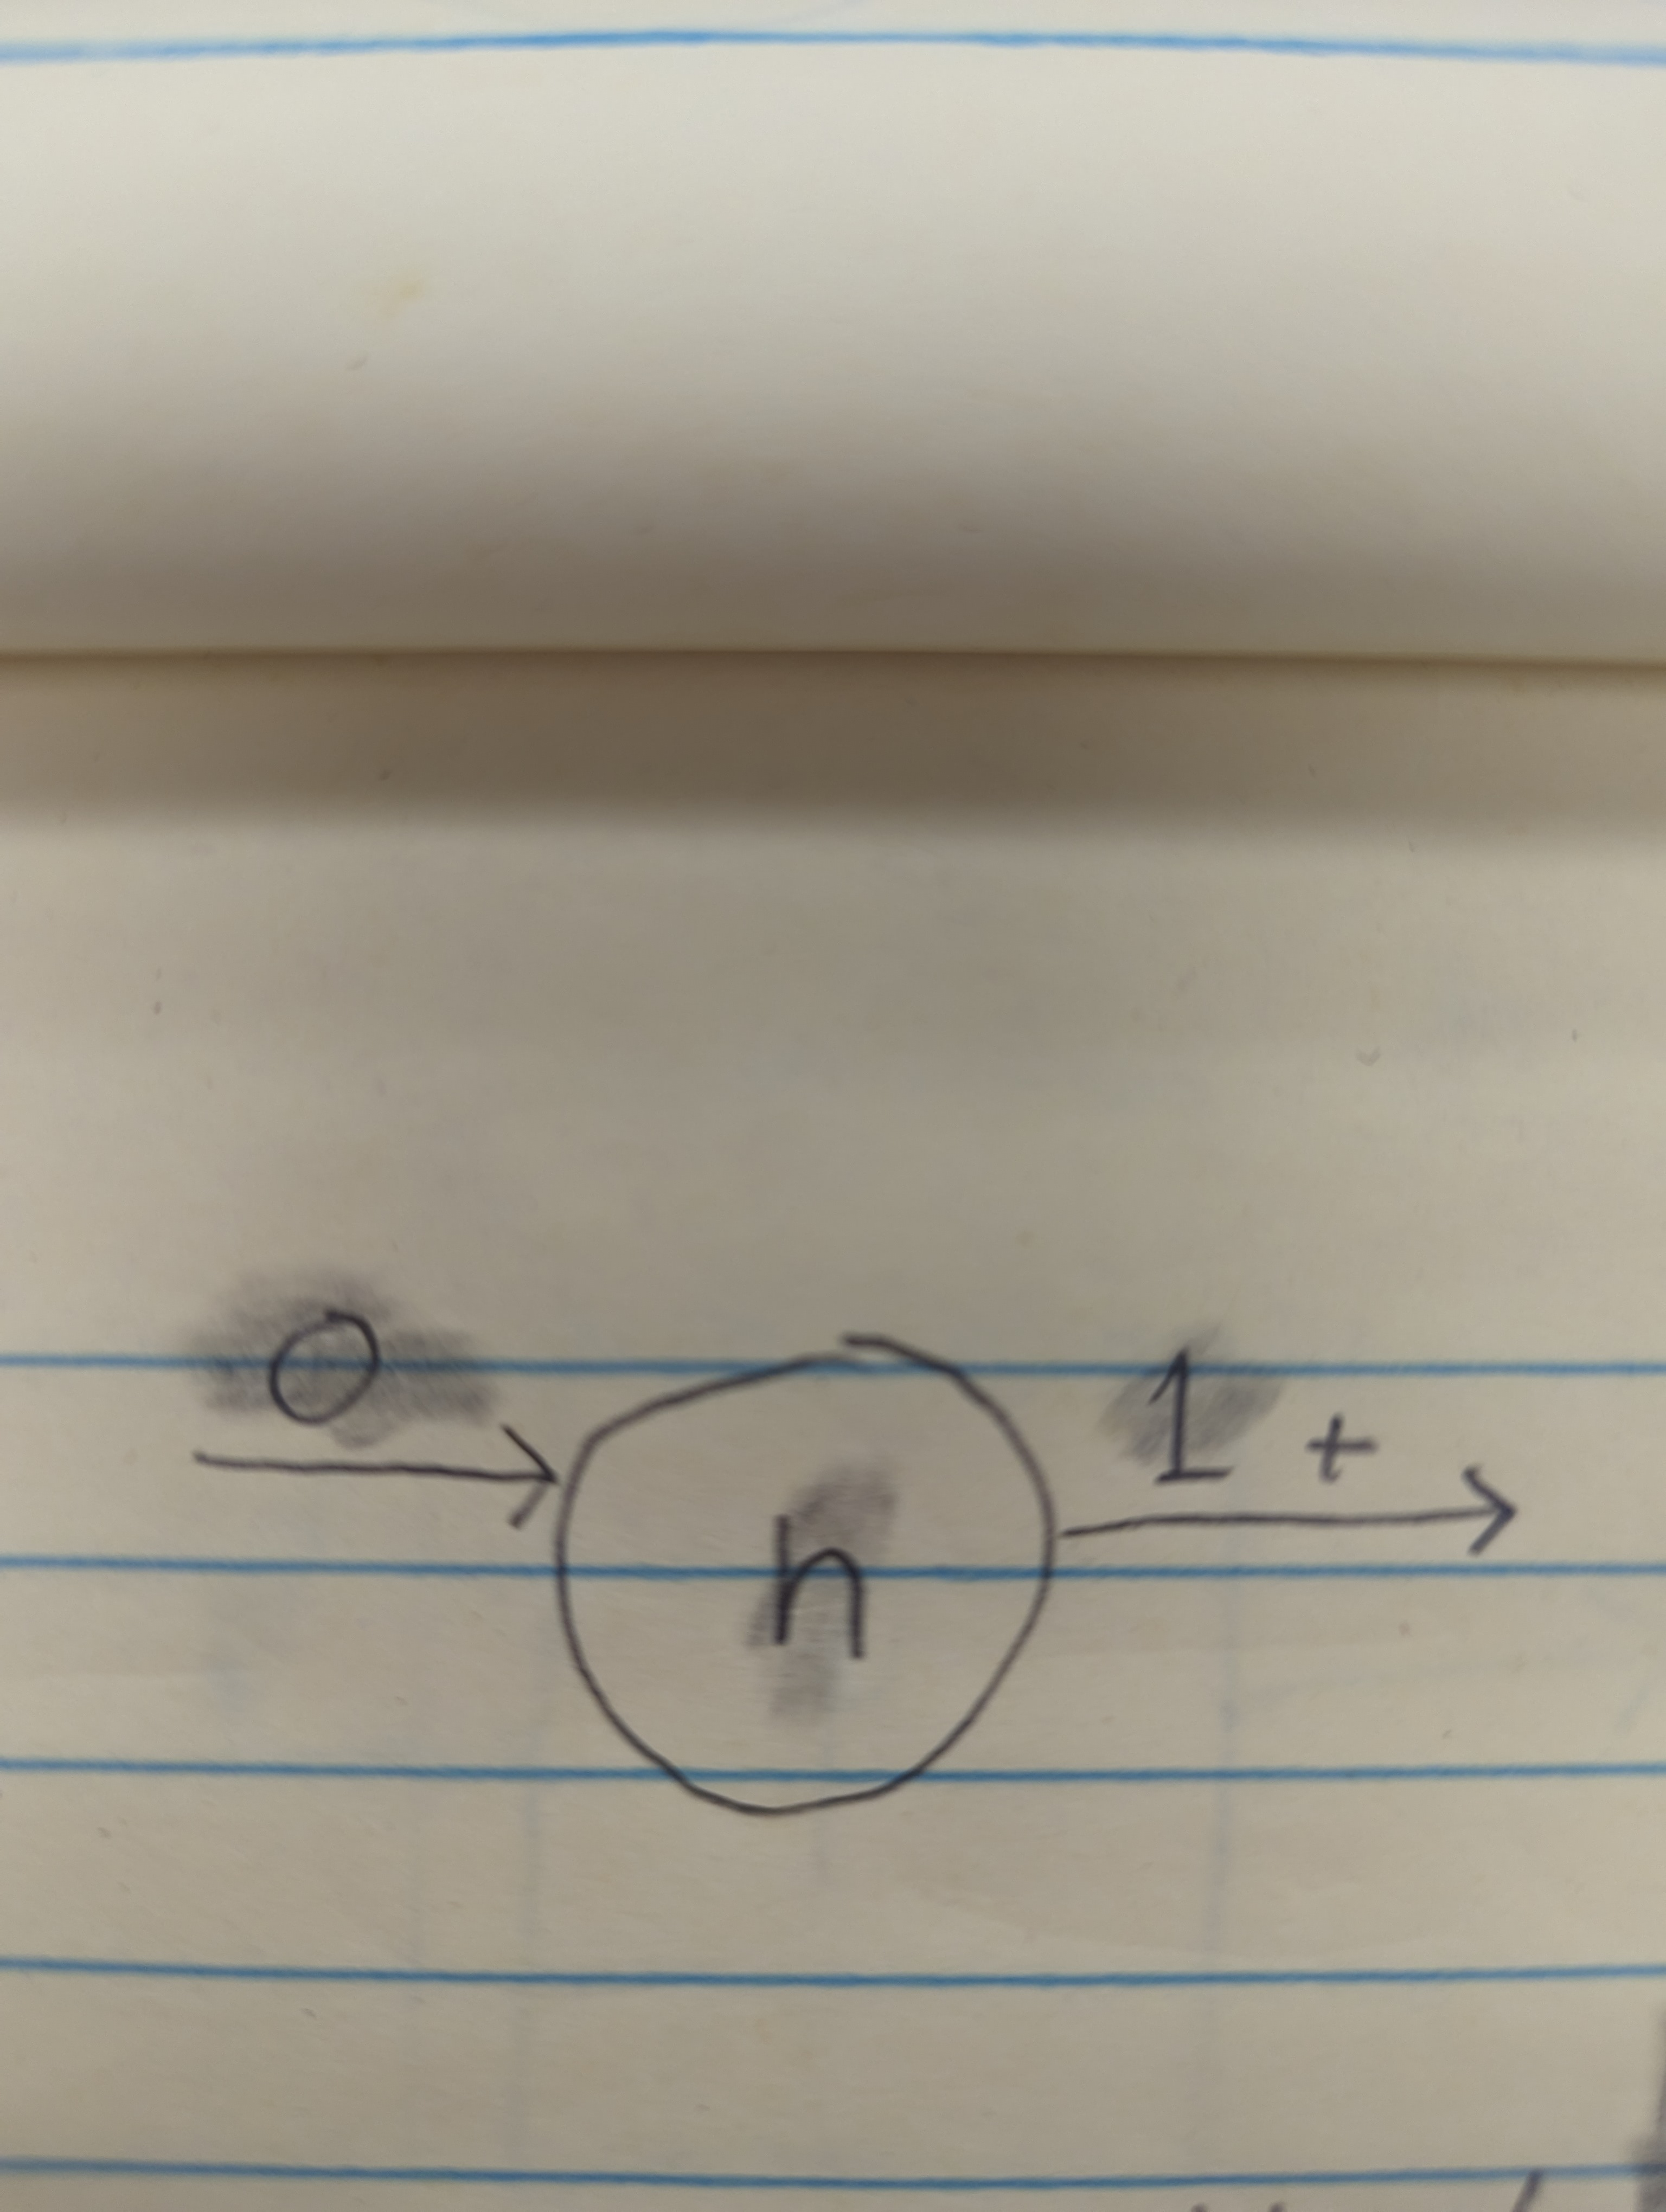
\includegraphics[width=\textwidth]{5}


\[ R_{003} \]
\[ \forall t \forall a (R_{t0a} \rightarrow R_{st1sa}) \]
\[ \therefore \exists t \exists a \R_{t1a} \]


\section*{Problem 6}

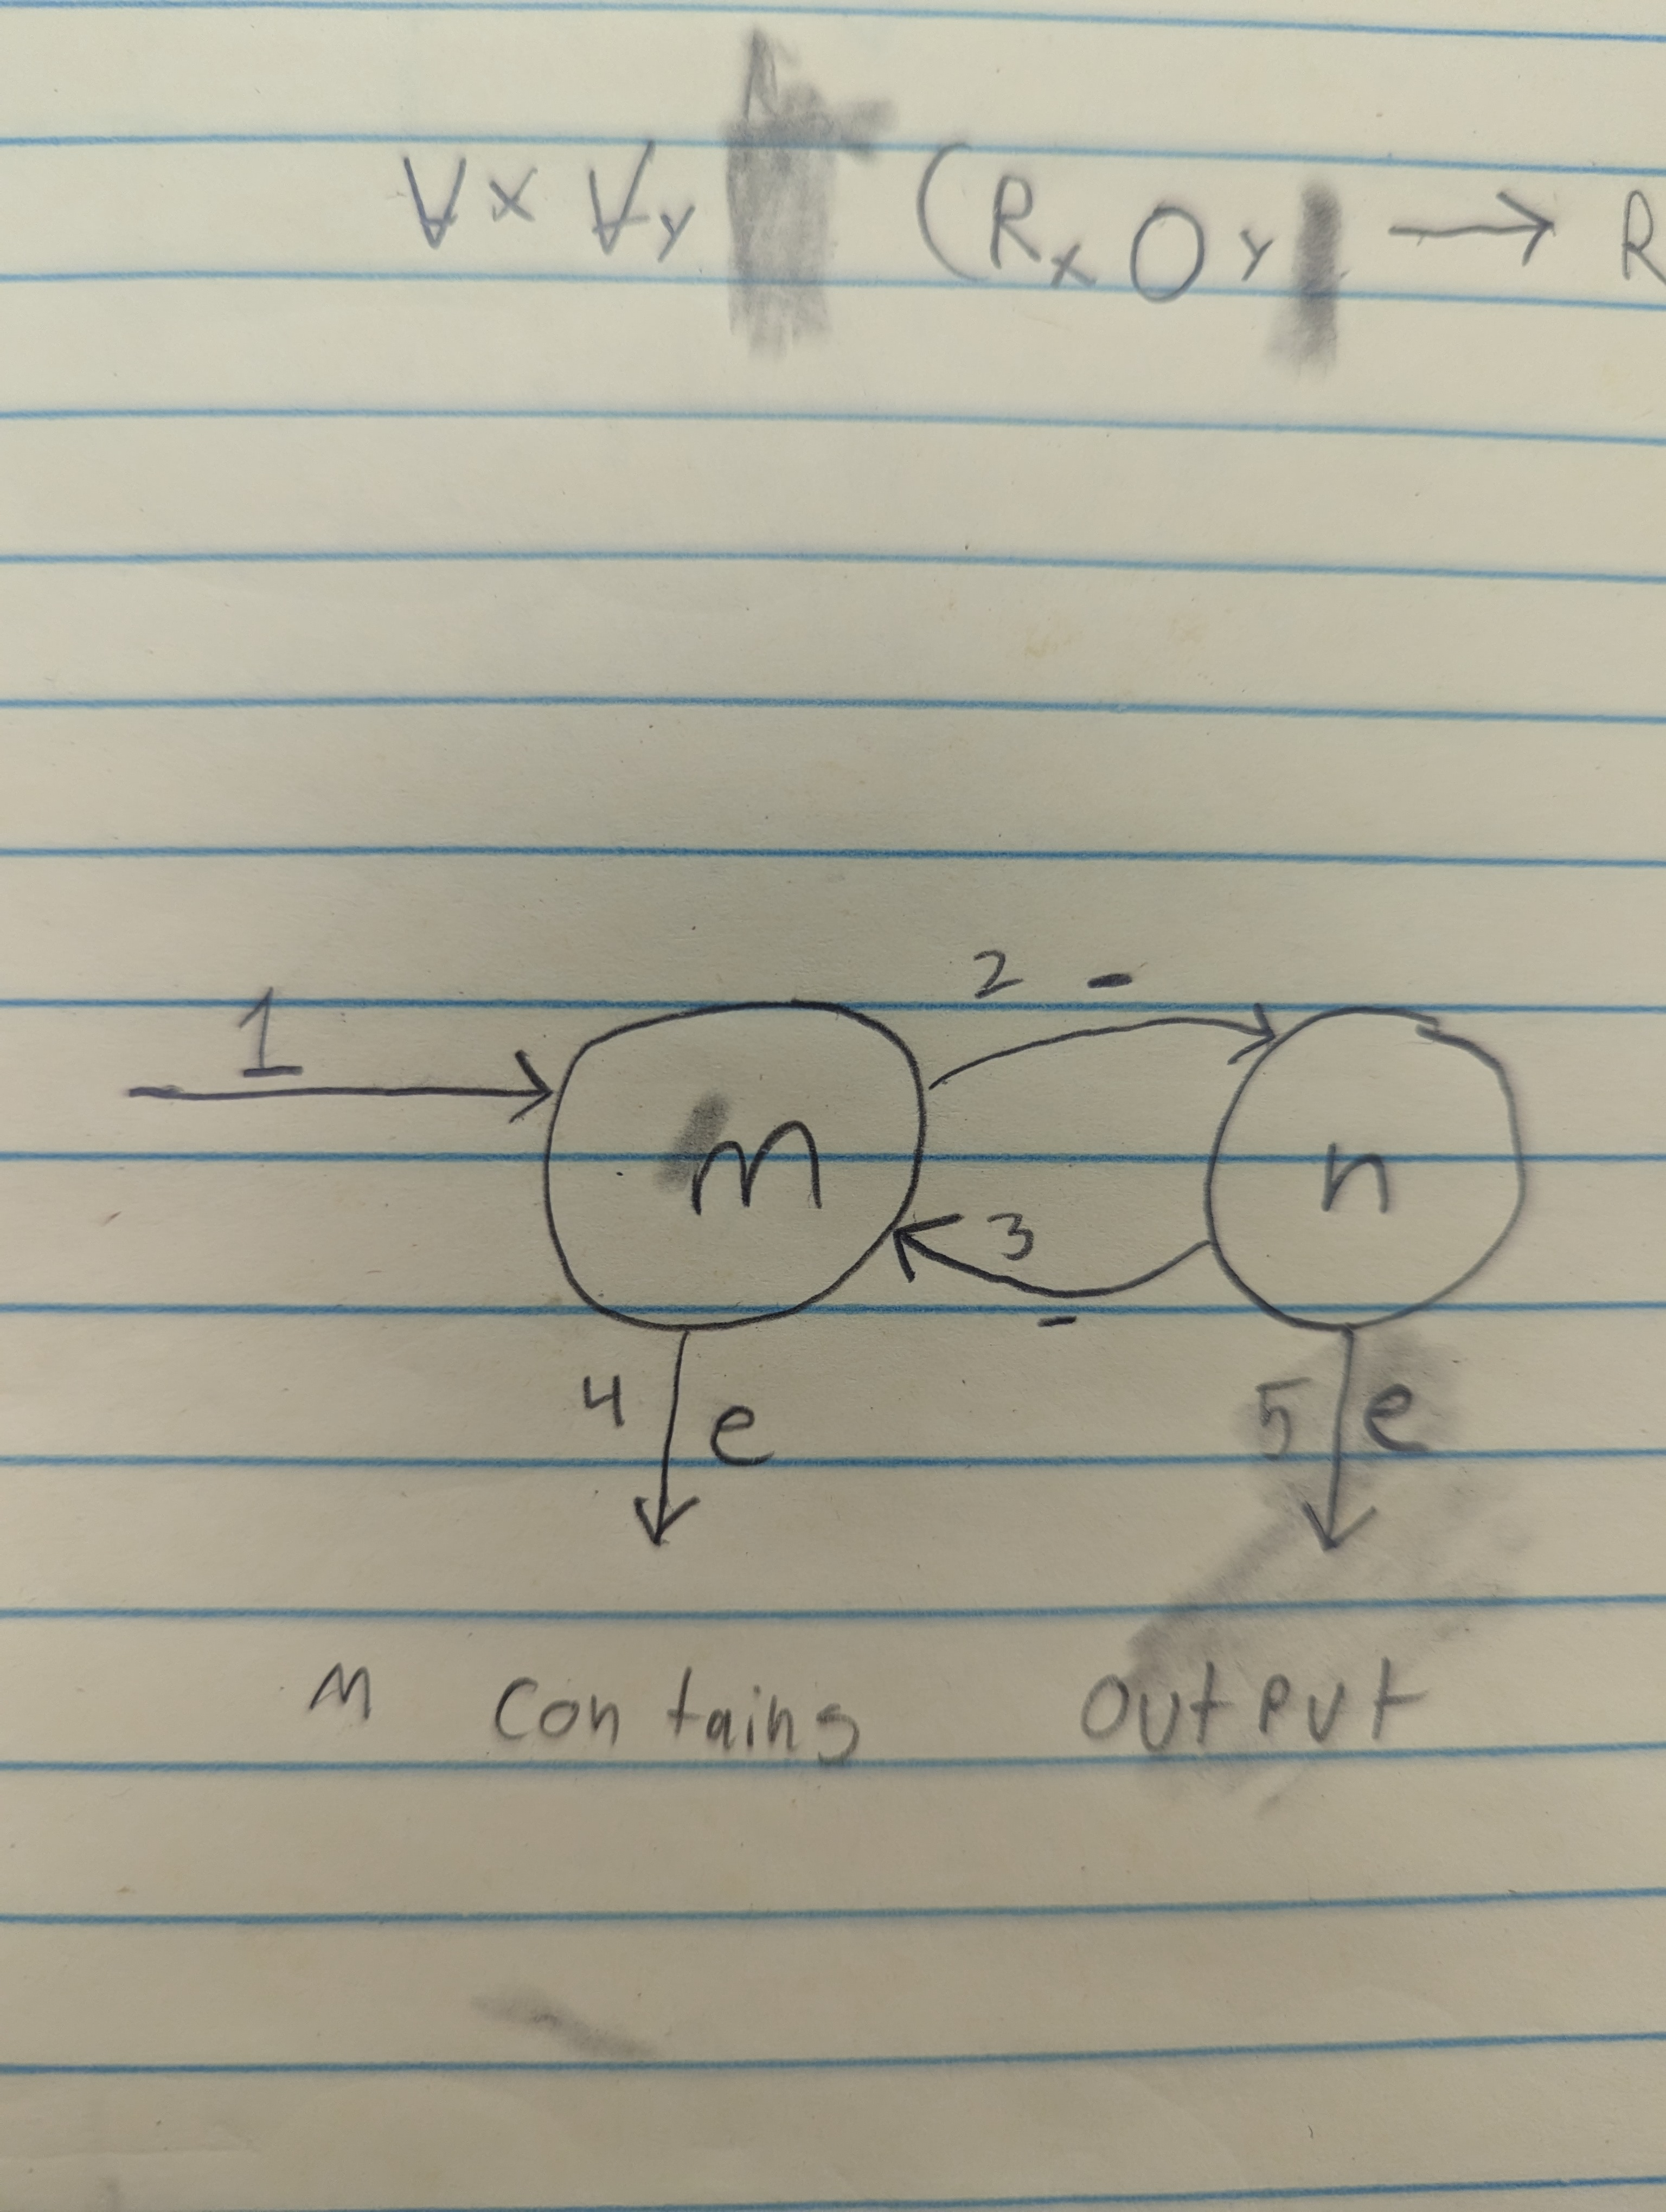
\includegraphics[width=\textwidth]{6}

\[ R_{0131} \]
\[ \forall t \forall m \forall n R_{t1smn} \rightarrow R_{t2mn} \]
\[ \forall t \forall n R_{t10n} \rightarrow R_{t40n} \]
\[ \forall t \forall m \forall n R_{t2msn} \rightarrow R_{t3mn} \]
\[ \forall t \forall m R_{t2m0} \rightarrow R_{t5m0} \]
\[ \forall t \forall n R_{t30n} \rightarrow R_{t40n} \]
\[ \forall t \forall m \forall n R_{t3smn} \rightarrow R_{t2mn} \]
\[ \therefore \exists t \exists m \exists n (R_{t4mn} \lor R_{t5mn}) \]

\section*{Problem 7}


\subsection*{Part A}
The self halting problem is a problem that asks if there exists a program that can be fed another program as input, and it will output true if the inputted program would halt if fed itself as input. 


\subsection*{Part B}

Let's assume that there is a program that can compute the self halting function called P. It outputs a 1 if the inputted program halts and a 0 if it doesn't. Now let's make a new program P* that uses P as a subroutine. P* first calls P with the input. If P outputs a 1, then P* will loop forever (not halt). If P outputs a 0, then P* will halt. 

P* is a contradictory program. If P* is fed P* as input, then P will have to make a choice on whether P* will halt, if it says that it doesn't halt, then it will halt, and vice versa. Thus, we arrive at a contraction, showing that P can not exist in the first place. 

\end{document}
